\chapter{G3 R\&D: Cold Radon Emanation}
\label{chap:chap7}

The use of ultra-radiopure materials is detrimental to the performance of a rare-event search experiment in its capacity to identify, characterise and assign a signal confidence to such rare searches. Furthermore, any hint of a signal in dark matter, neutrinoless double beta decay, or other such rare-searches are modeled against the expected background model, which must be accurately characterised. Radon emanation has emerged to be the most important background limiting the science capability of direct detection G2 experiments such as LZ and XENONnT, despite the screening efforts to date. Future experiments, such as a planned LXe G3 dark matter experiment, will need to control radon backgrounds by a further order of magnitude to achieve a sub-dominant radon level, while opening up avenues for new rare searches. Although screening facilities for radon emanation exist, none of these are capable of assessing radon emanation at cryogenic temperatures, important to experiments such as LZ or future LXe G3, in building reliable and accurate background models. The RAL cold radon emanation facility, detailed in this chapter, is an attempt to study radon emanation from a variety of detector material, to model emanation via recoil and diffusion as a function of temperature.
 
 
%%------------------------------$$
\section{Motivation}
\label{sec:motivation_7}
%%------------------------------$$

Emanation of \RnTTT{} from detector material and its subsequent decays, as detailed broadly in chapter \ref{chap:chap4}, is now the leading background contributor to current generation dark matter detectors in search for WIMPs. The concentration of \RnTTT{} in past LXe experiments have been declining as a result of more extensive screening campaigns and scaling, with reported activities of 65 \uBqkg{} in XENON100 \cite{Aprile:2012nq}, 32 \uBqkg{} in LUX \cite{Akerib:2013tjd}, 22 \uBqkg{} in PandaX-I \cite{Xiao:2014xyn}, 9.8 \uBqkg{} in XMASS \cite{Abe:2013tc}, and ($3.65\pm0.37$) \uBqkg{} in EXO-200 \cite{Albert:2015nta}. The projected radon emanation activity for the LZ experiment is given as 1.81 \uBqkg{}. The improvement in radon activity in LZ over its predecessor, LUX, is associated with the dedicated radon screening campaign \cite{lz_screening} and the increase in volume-to-surface ratio of LXe within the detector; despite these improvements, radon emanation is projected to be the largest background contributor in the ER band and in the WIMP ROI, limiting the reach of the experiment. 

With second generation dual-phase LXe detectors approaching data taking, there is now an effort to envision the continuation of this technology to probe WIMP-nucleon cross sections to a few $10^{-49} \; \MathText{cm}$, exploring the remaining parameter space down to the \textit{neutrino floor}. However, the radon emanation rates currently achieved, although suppressed to unprecedented levels, are already limiting the science capabilities of G2 experiments. Future G3 experiments, as demonstrated with the toy detector in chapter \ref{chap:chap6}, will have to reduce radon backgrounds by a further order of magnitude, where concentrations of $\sim 0.1$ \uBqkg{} of radon must be achieved in order to probe down to cross sections of $\sim10^{−49} \; \MathText{cm}$ \cite{Schumann:2015cpa}. Furthermore, in reducing the radon background to sub-dominant levels in comparison to neutrino backgrounds, new physics capabilities open up within the ER band of such experiments \cite{Schumann:2015cpa}. A precise measurement of the \textit{pp}-neutrino flux will allow for testing the standard solar model (SNO), and can lead to a better understanding of neutrino production and the main energy production mechanism in the Sun \cite{Aalbers:2016jon}. \textit{pp}-neutrino and \BeS{} neutrinos are estimated to make up more than 98\% of the total neutrino flux from the sun. Nevertheless, achieving a low radon level will be the largest background reduction challenge for a G3 experiment, where studies on radon emanation at cryogenic temperatures, novel radon diffusion suppression techniques and online radon removal from LXe will be required to better understand, model and mitigate for radon emanation. 

One of the largest sources of uncertainty in modeling the radon emanation concentration within LXe detectors is the lack of data on the properties of radon emanation at operational temperatures (-97.4$^{\circ{}}$C for LZ). The best and worst case estimates of radon emanation in LZ is projected at 11 mBq and 60.8 mBq in total, respectively; driven from room temperature measurements of detector material and cold suppression coefficients based on various other noble gas studies \cite{Schowalter_2010}. Facilities that provide high sensitivity radon emanation assays are rare and to-date only perform measurements at room temperatures. With gaseous radon turning into a liquid at -62$^{\circ}$C and into a solid state at -70$^{\circ}$C, there remains a large uncertainty on how this monatomic gas behaves and diffuses through material when exposed to LXe temperatures. Although the fraction of emanation due to recoil upon the \alpha{}-decay of \RnTTT{} is expected to be unaltered, diffusion of \RnTTT{} and gases within solids in general are known to depend on temperature. If the diffusion coefficient substantially changes going from room to LXe temperature, this may give enough time for \RnTTT{} to decay ($\tau_{1/2}=3.82 \; \MathText{days}$) within the material before mixing out into the active LXe, suppressing the background contribution of radon emanation.

The diffusivity, $D$, of a gas through a solid is dependent on the permeability, $K$, given as
%
\begin{equation}
    K = Db,
    \label{eq:permeability}
\end{equation}
%
where $b$ represents the solubility of gas in the material, determining the concentration of gas dissolved in the material at a given partial pressure; whereas diffusivity determines the rate at which gas flows in the material. Experimentation of permeability is often achieved by constructing a thin film of material. A concentration gradient is set up on either side of the sheet; where permeability of a given gas can then be determined through the observation of the time evolution of gas permeation through the film. The dynamics of the flow are determined only by the thickness of the membrane, $d$, and diffusivity. For such a setup, a breakthrough time is defined as the time taken for a significant amount of gas to permeate through the film, where
%
\begin{equation}
    t_{b} = \frac{d^{2}}{6D}.
    \label{eq:breakthrough_time}
\end{equation}
%
Furthermore, permeability and breakthrough time for noble gases through materials are expected to increase with temperature, and assumed to follow the relations \cite{Schowalter_2010}
%
\begin{equation}
    &K(T) \propto exp\left(\frac{-E_{K}}{k_{B}T}\right), \\
    \vspace{5mm}
    &t_{b}(T) \propto d^{2}exp\left(\frac{-E_{D}}{k_{B}T}\right),
    \label{eq:perm_breakthrough}
\end{equation}
%
where $E_{K}$ is the energy of permeation, and $E_{D}$ is the energy of diffusion. However, it's important to note that, although such experimental setup's can further the understanding of permeability and the effect of temperature on diffusivity, radon emanation from material emerge from the constant formation of \RnTTT{} from its parent isotope of \RaTTS{}. Hence, in order to fully understand how emanation changes as a result of temperature, a preliminary understanding of the concentration of \RaTTS{} or \UTTE{} and its distribution across the material is also required. Furthermore, although \cite{Schowalter_2010} demonstrates experimentally that permeability does indeed follow the relationships given in equations \ref{eq:perm_breakthrough} with increasing temperature beyond room temperature, it does not, however, demonstrate this behaviour at much colder temperatures, were liquefaction and solidification takes place.

To focus on developing a further understanding of radon emanation through detector material and its temperature dependence, a cold radon emanation facility (CREF) capable of measuring radon emanation to lower sensitivities than previous achieved by the operational setup detailed in chapter \ref{chap:chap4} was envisioned. The following sections will outline the design of the facility currently under construction and its operational procedures in becoming a leading laboratory for studying radon in line with the ambitious goals set out for a future G3 LXe observatory. This ambitious project, spanning beyond this thesis, will aim to better understand the recoil and diffusive emanation ofd radon in a temperature range between 77K to room temperature and above; study novel barrier materials and chemical treatments of surfaces to reduce backgrounds from radon emanation and radon plate-out; and eventually study radon filtration techniques, such as low-temperature vacuum swing absorption, as detailed in \cite{Street:2017bde}. 


%%------------------------------$$
\section{CREF Design}
\label{sec:radon_design}
%%------------------------------$$

The CREF facility presently under construction is situated at the 
Rutherford Appleton Laboratory (RAL) within a ISO6 cleanroom. Although it is currently not operational, many parts of the system are under development in tandem. The conceptual design of CREF heavily relies on the UCL system described in chapter \ref{chap:chap4} with some divergences due to the necessity of cold emanation measurements. The schematic diagram of CREF, demonstrating the piping and the instrumentational layout, designed to maximise operational flexibility is shown in figure \ref{fig:cref_pid}.
%
\begin{figure}[h!]
    \centering
    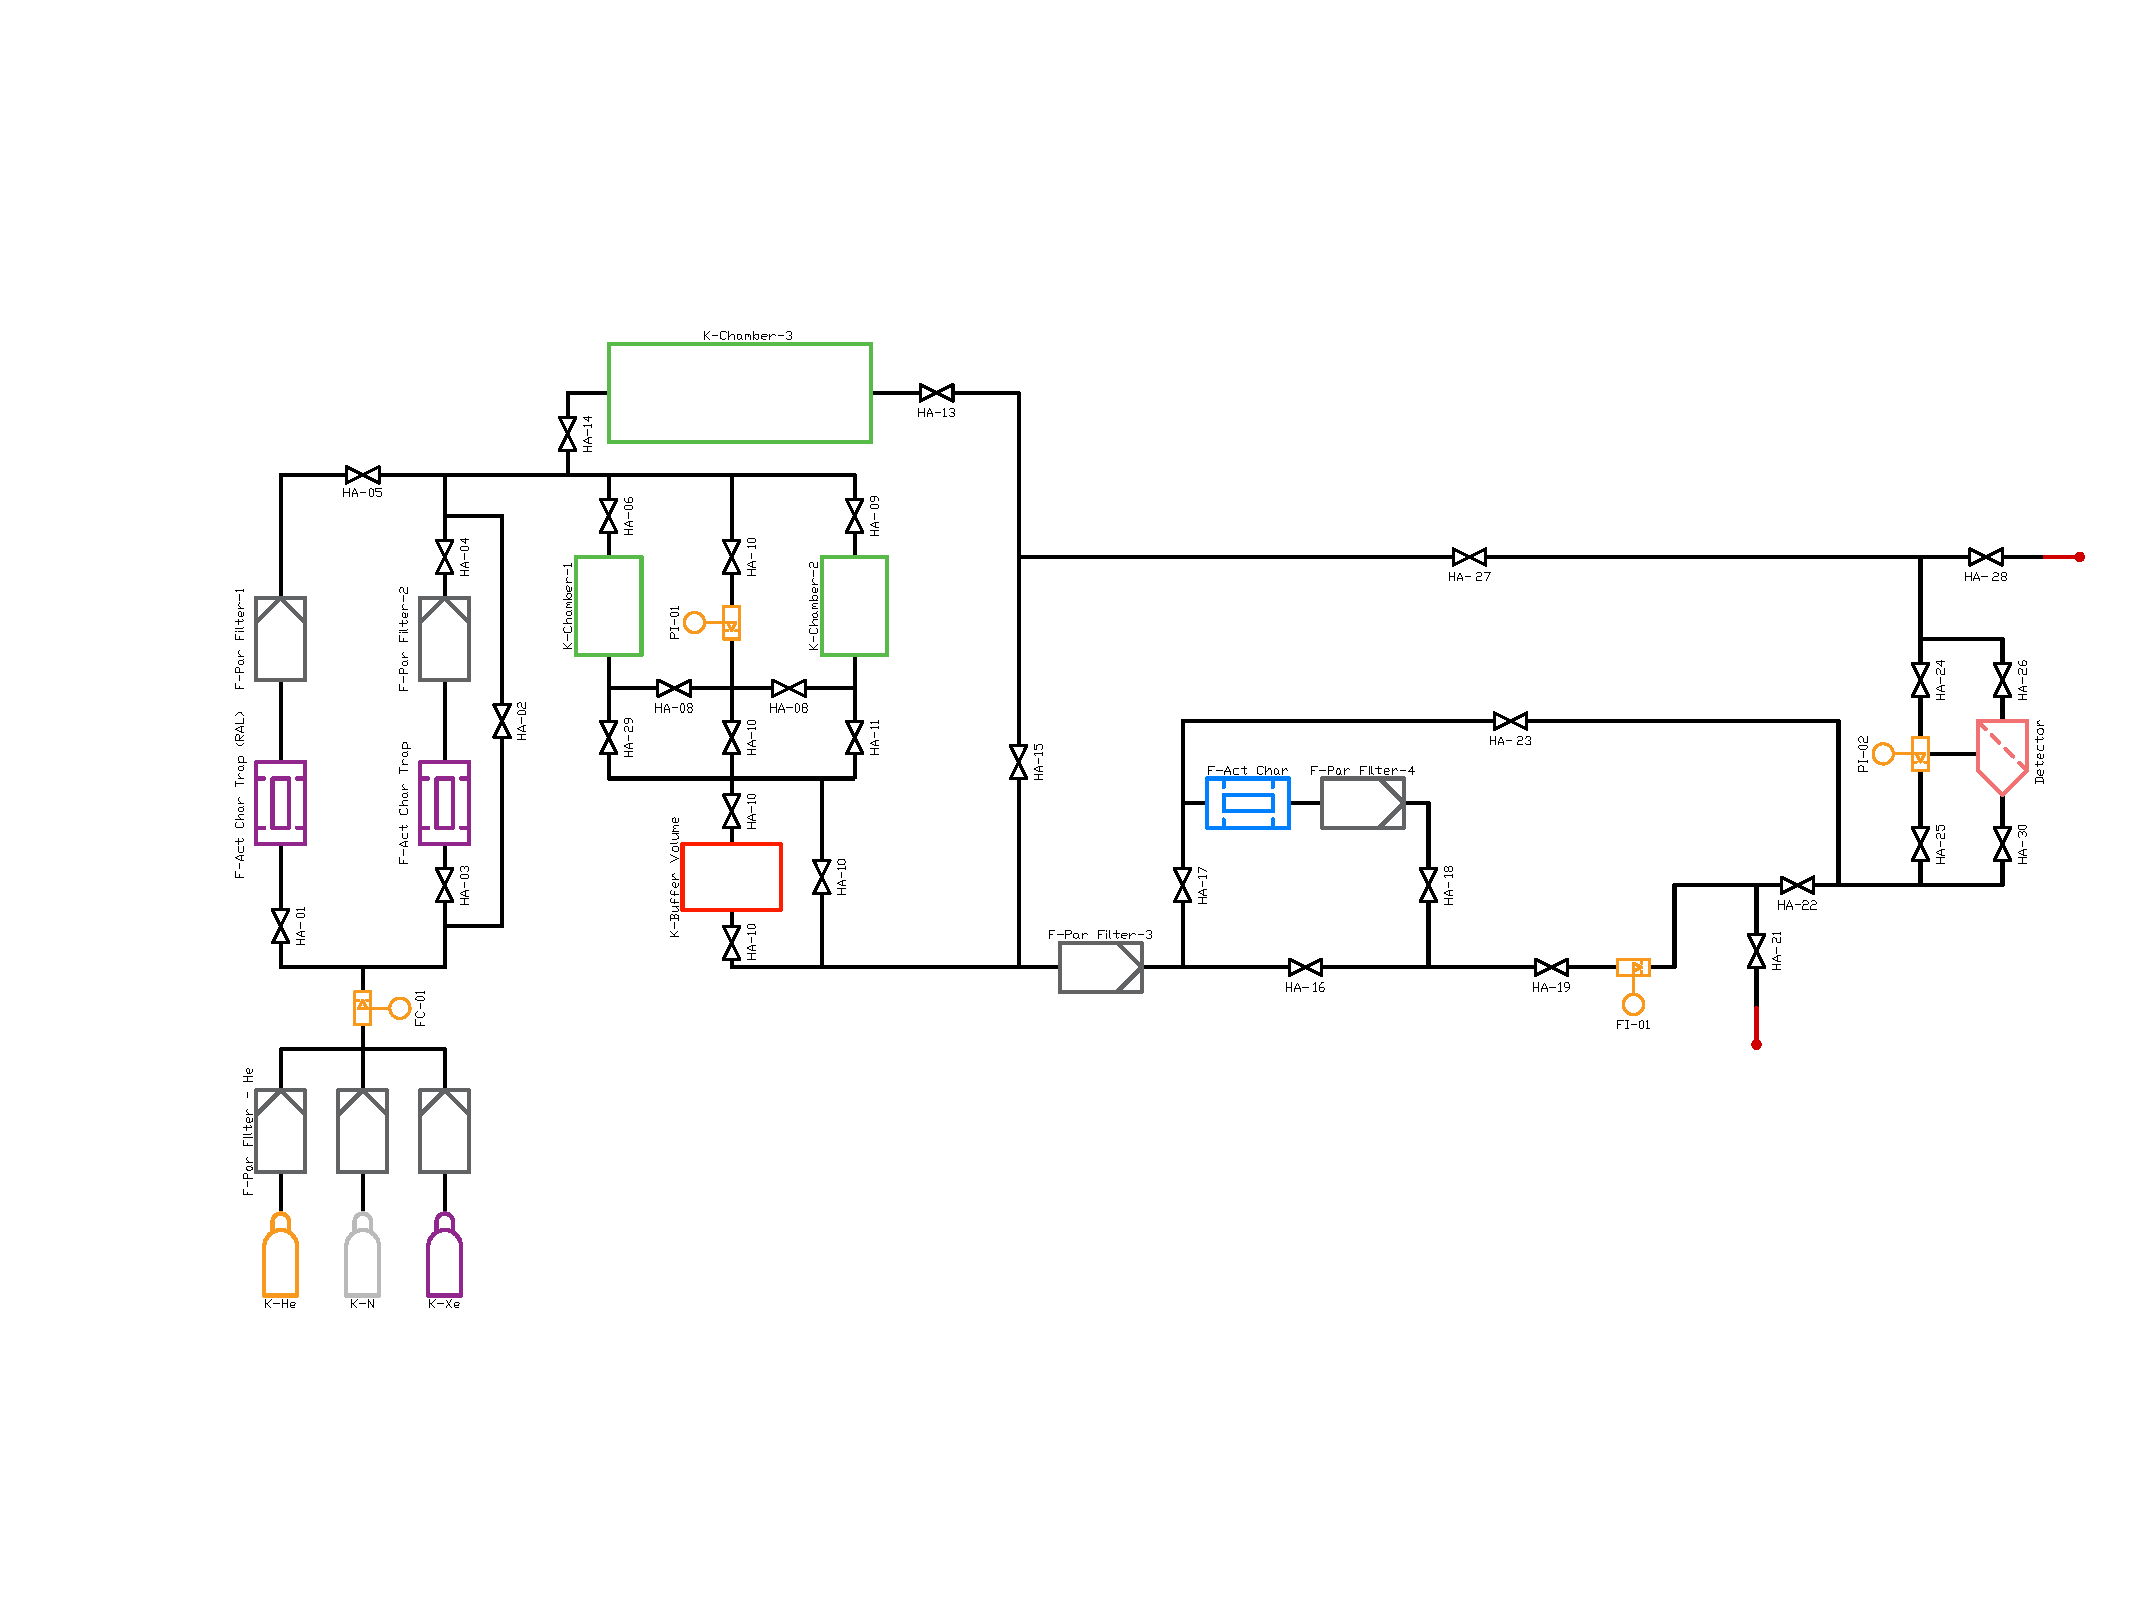
\includegraphics[scale=0.5]{Chapter_7/Figures/cold_radon_pid.pdf}
    \caption[Schematic diagram of the CREF gas system flow path.]%
    {Schematic diagram of the CREF gas system flow path.}
    \label{fig:cref_pid}
\end{figure}
%

The idea behind the system design is to facilitate a high degree of flexibility in operation, with the ability to use different carrier gases, varying sizes of emanation chambers, and the ability to measure radon through a 1-step and a 2-step transfer mechanism. Chambers 1 and 2 are planned to have a volume of $\sim2.7$ L, similar to those operated by the UCL radon system. These will be used for precise radon emanation measurements from smaller samples, where room temperature and cold measurements can be performed. The internal radon emanation background from the chambers is proportional to the surface area, hence smaller surface area will allow for more precise measurements. The small emanation chambers will be cooled using an immersion cooler (Thermo Scientific EK90 LT3291901) with a temperature range of -90$^{\circ}$C--40$^{\circ}$C. The third chamber (\textit{Chamber-3}) in figure \ref{fig:cref_pid} is a much larger emanation chamber, with a volume of $\sim200$ L, operating within a 500 L cryogenic temperature vessel, capable of cooling down to $\sim77$ K. This chamber will be used to hold much larger samples and instrumental systems of a future G3 experiment for more accurate emanation assays. Due to its much large volume, harvesting radon from a volume of this size has to be done through a 2 step transfer mechanism; due to the limitations on volume and pressure of the detection chamber. The emanated radon atoms are first flowed through a radon concentration line, where the radon in the gas is captured by an activated charcoal trapping unit (CarboAct \textit{High-Purity Activated Charcoal}, 0.4--2.0 mm). The radon concentration unit, labeled as \textit{Act Char}, is initially kept at LN temperatures to increase trapping efficiency, and later, heated up so to release the trapped radon, which is transferred into the detection chamber via the carier gas. A pictorial diagram of the large cryogenic chamber setup is shown on figure \ref{fig:cref_cryogenic_chamber}.
%
\begin{figure}[h!]
    \centering
    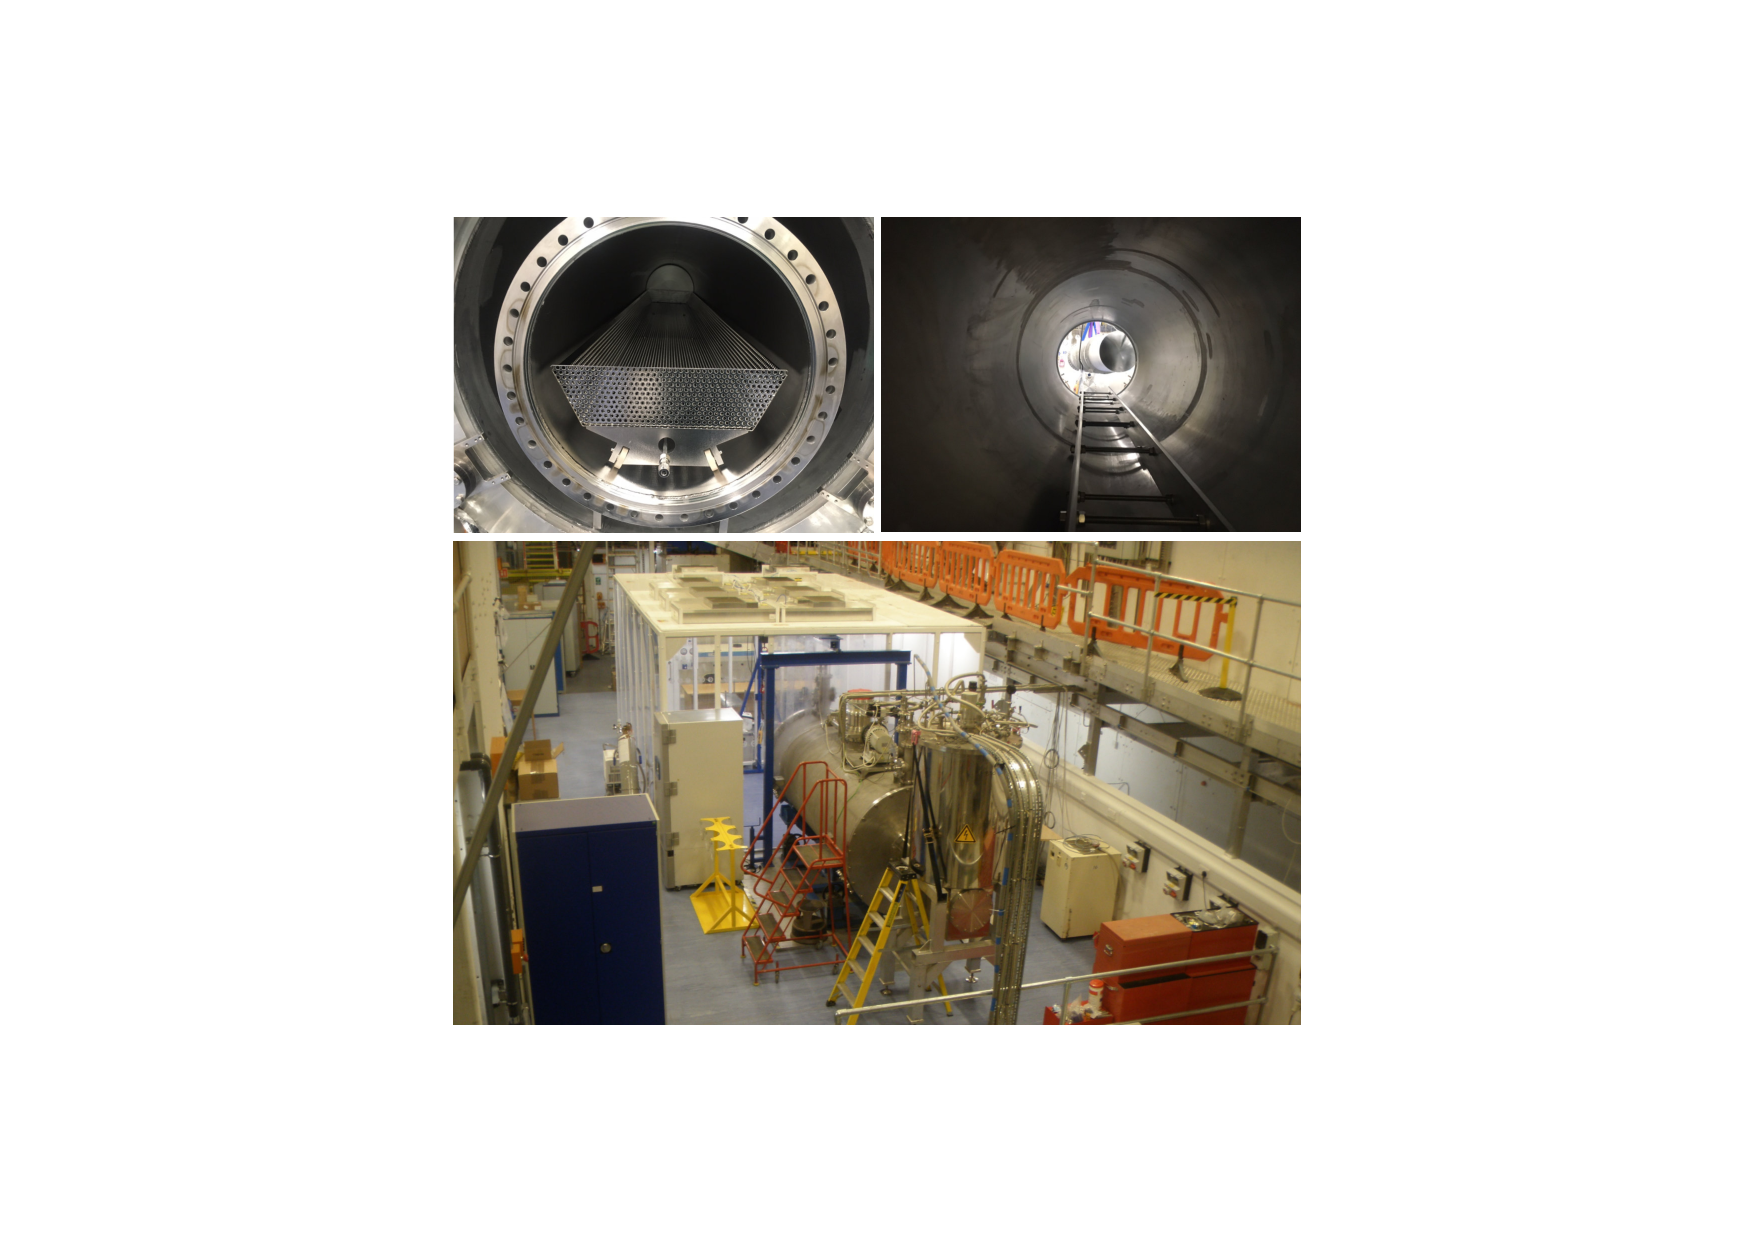
\includegraphics[scale=0.78]{Chapter_7/Figures/cryo_cooler_chamber_and_lab.pdf}
    \caption[Pictorial diagram of the large cryogenic chamber used in CREF.]%
    {Pictorial diagram of the large cryogenic chamber used in CREF. The above two images show the inside of the cryogenic vessel, whereas the image below shows a broader angle of the cryogenic system and its connection to the CREF cleanroom.}
    \label{fig:cref_cryogenic_chamber}
\end{figure}
%

To achieve lower background levels, it is vital that the carrier gas used within such system is radon-free. As radon is constantly produced in minute quantities, naturally, the carrier gas is contaminated with radon to varying degrees. The CREF gas panel incorporates a radon removal system, constructed from cylinders of activated charcoal and kept inside an ultra-low freezer (Thermo Scientific TLE30086V) operating at -80$^{\circ}$C. Labeled as \textit{Char Trap}, the carrier gases will initially go through 0.5 micron particle filters to remove any particulate matter that may otherwise contaminate the gas system and then through the charcoal traps for radon removal. Such a system can be used indefinitely with little or no deterioration in performance, as the trapped \RnTTT{} atoms decay away rapidly due to relatively short half-life. Although this setup has been demonstrated to work well with helium and nitrogen, there remains uncertainty on its effectiveness with alternative gas carriers, such as argon or xenon, that require further investigation. 

Furthermore, the flow rate of the carrier gas is another variable that is vital in calibrating the system and in assuring repeatability across multiple sample measurements. Often, the detector is calibrated under a set amount of the carrier gas, with the aim to operate under the same pressure for all samples. Moreover, in calibrating the detector, a \RaTTS{} calibration source with known activity is used. The source is initially sealed to allow for \RnTTT{} to build-up, which is then transferred into the detector by using the carrier gas, where the flow time, $t_{f}$, determines the activity of \RnTTT{} transferred into the detector. The precision and accuracy of the gas flow directly impacts the precision and accuracy of the detection efficiency. The precise control of the gas flow is achieved through a multi-gas/range mass flow controller (MFC) (MKS Instruments \textit{P9B}). The MFC is capable of $<750$ ms control time and accuracy to within 1\% of set point. 

The end result of harvesting radon at varying temperatures from the chambers specified above will be to determine the activity of radon that has emanated into these volumes. This will be achieved through the use of an ultra-pure high-sensitivity radon detector. The detector utilised by CREF has been developed by The University of Tokyo (UoT) and operates under the same principles as detailed in section \ref{secsec:electrostatic_detector}). The electrostatic detector constitutes an 80 L vessel with a PIN-photodiode detection unit, used to capture and detect the \alpha-particles from the decays of \PoTOE{}, \PoTOF{} and various other isotopes in \RnTTT{} and \RnTTZ{} sub-chains. The observed rates of \PoTOE{} and \PoTOF{} will then be used to reconstruct the radon emanation rate. The background radon levels of the detector is expected to be lower than that operated by UCL, due to the use of knife-edge flanges with metal gaskets to seal the detector, in comparison to the acrylic plate and Viton O-rings that were used in the 70 L radon detector. This modification has led to an improved vacuum level of the vessel, capable of achieving $10^{-4}$ Pa, as measured by the UoT team on an identical detector to that procured for the CREF project \cite{Hosokawa:2015koa}. A pictorial diagram of the 80 L PIN-diode detector is shown in figure \ref{fig:cref_detector}.
%
\begin{figure}[h!]
    \centering
    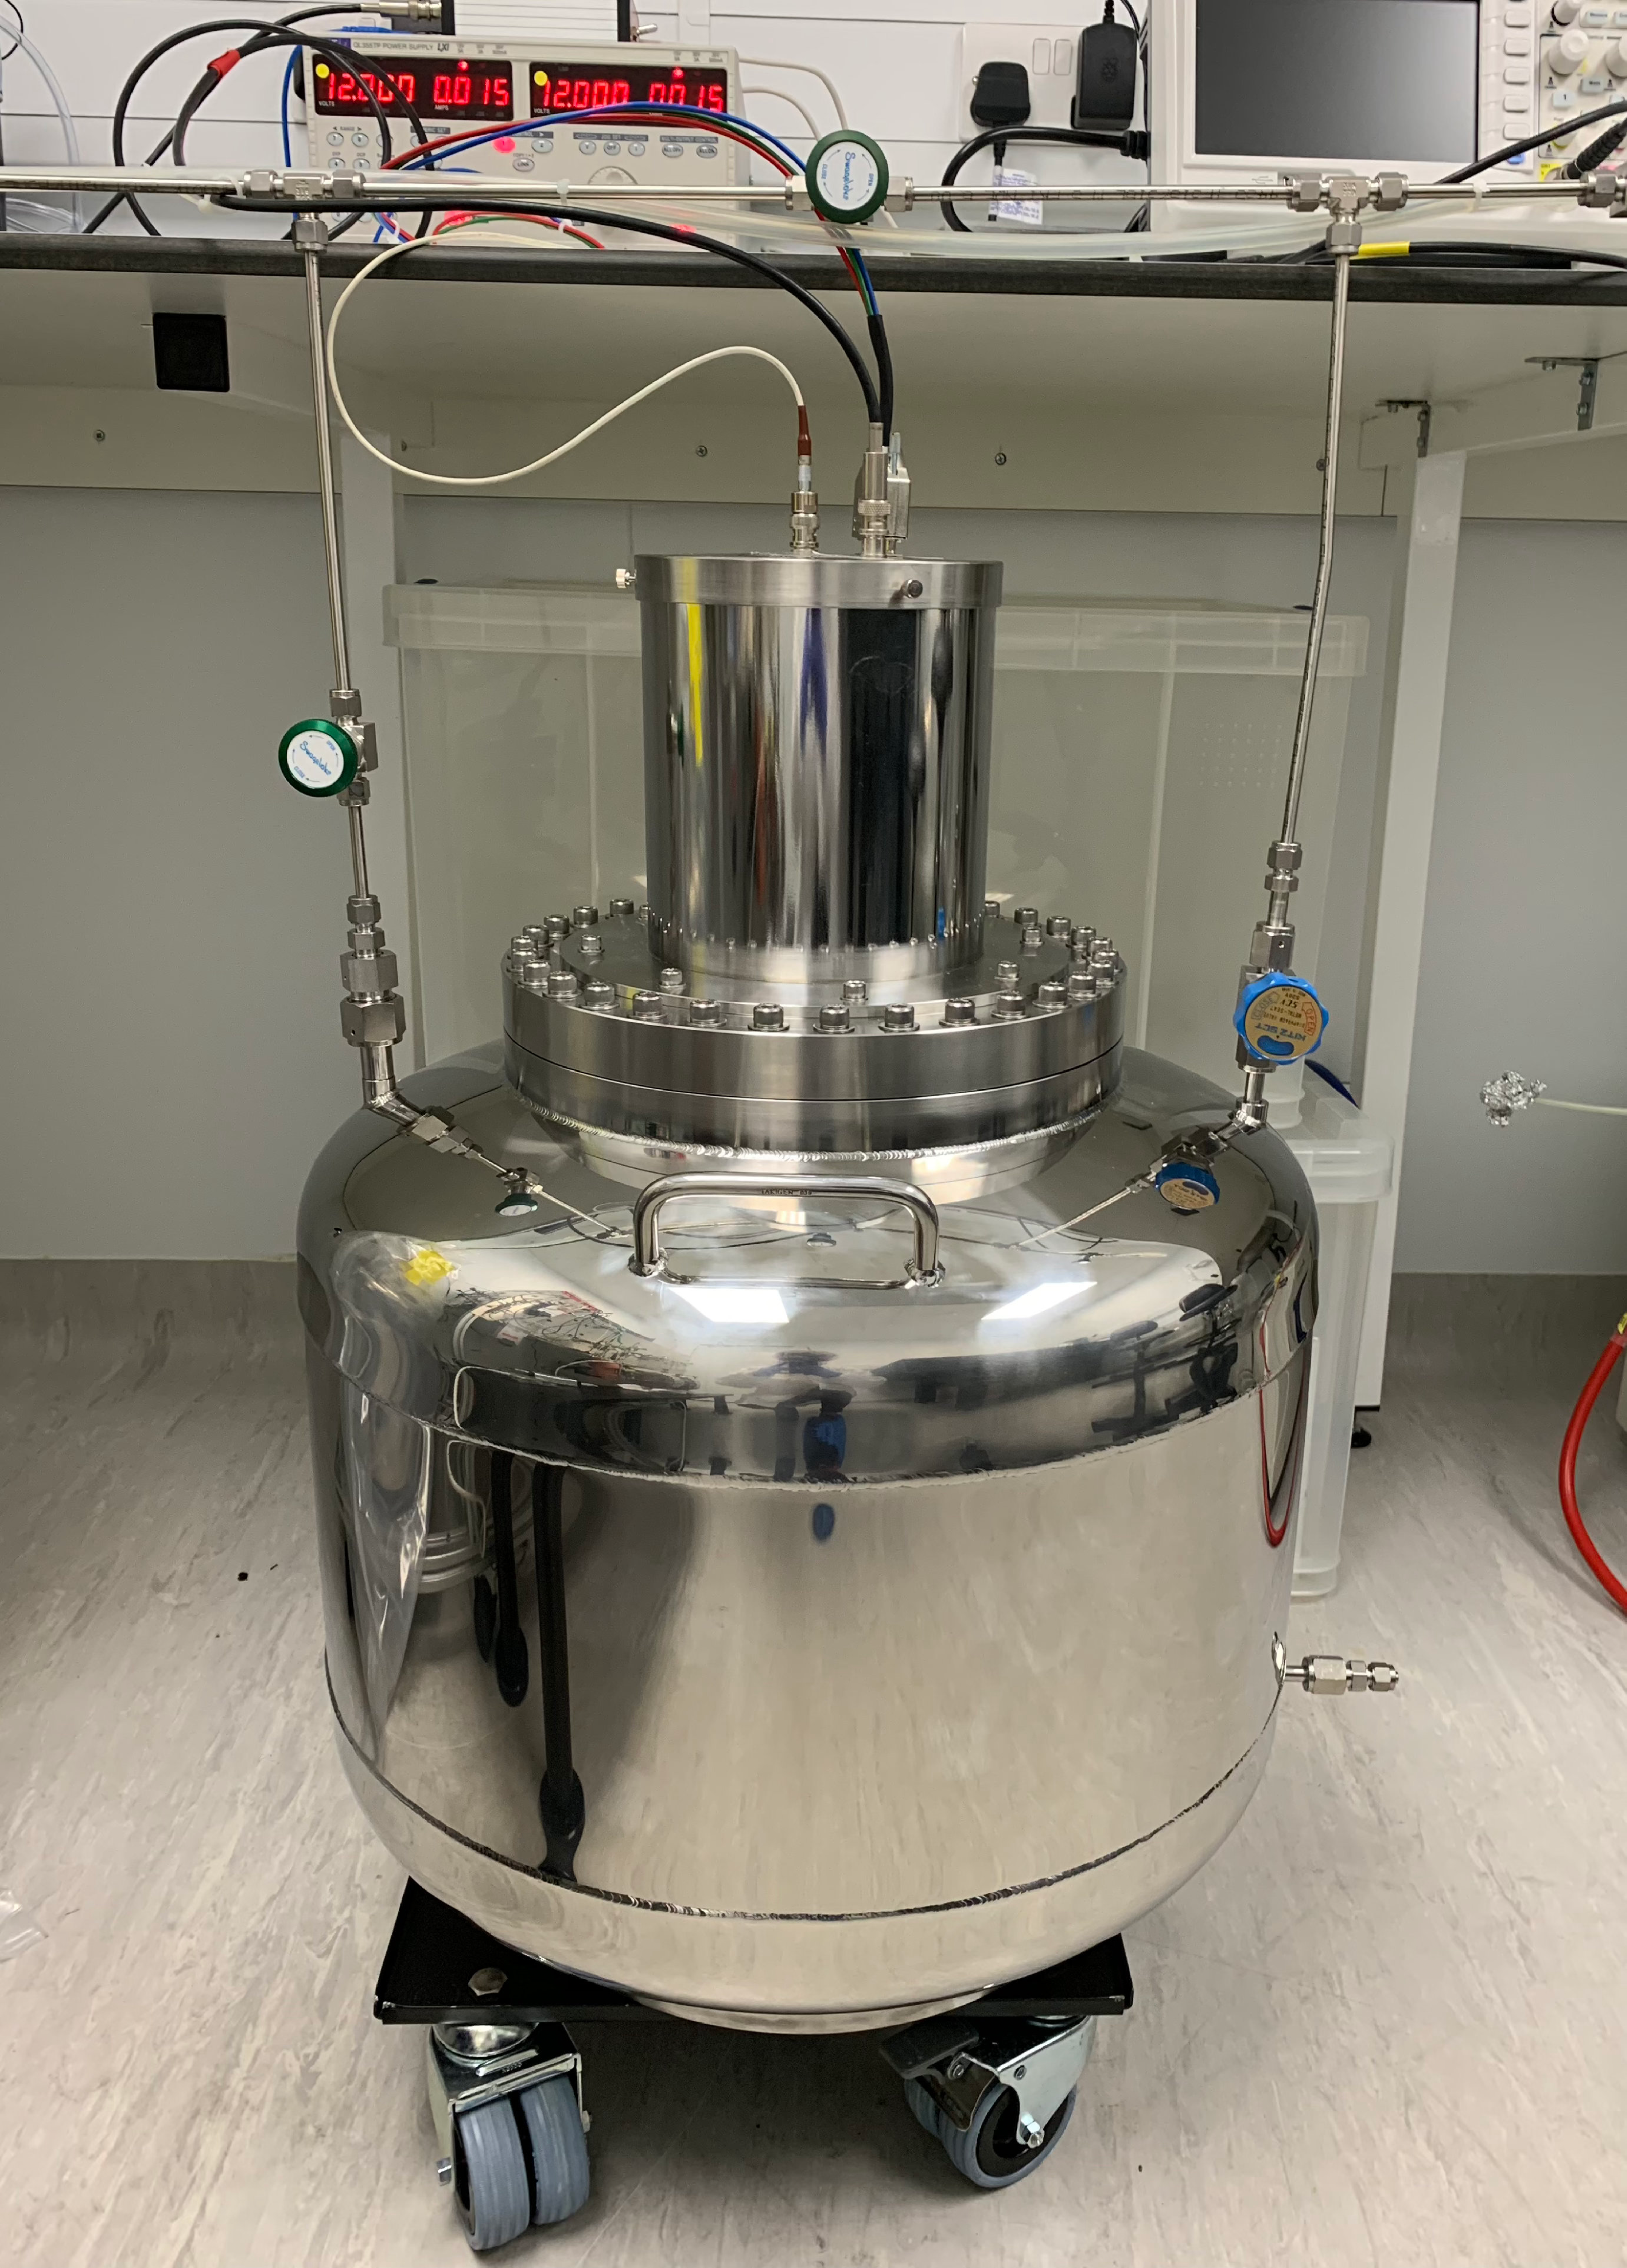
\includegraphics[scale=0.1]{Chapter_7/Figures/detector_image.pdf}
    \caption[Pictorial diagram of the 80 L high-sensitivity PIN-diode radon detector.]%
    {Pictorial diagram of the 80 L high-sensitivity PIN-diode radon detector.}
    \label{fig:cref_detector}
\end{figure}
%

The detector consists of an 80 L stainless steel vessel, with the inner surface of the vessel electropolished to a roughness of less than 0.8 \micro{}m to remove surface contaminants and decrease surface roughness; both of which can contribute to internal radon emanation backgrounds. The PIN-photodiode (HAMAMATSU \textit{S3204-09}) is connected to a ceramic feedthrough, mounted on the top flange of the vessel and offset by 5 cm from the bottom of the flange. The PIN-diode with dimensions 18 mm x 18 mm, has its window removed to reduce energy loss as the \alpha-particles decay towards the photodiode. In operational mode, the p-layer of the PIN-diode is biased at -1.9 kV, while the vessel is held at ground. In addition, the high-voltage feedthrough uses high-purity alumina (\alumina{}) to reduce internal radon emanation background originating from the detector volume; an improvement on its predecessor detailed in chapter \ref{chap:chap4}. Although an identical radon detector build by the UoT team has been characterised in detail and used by the Super-Kamiokande experiment for radon emanation measurements \cite{Hosokawa:2015koa, Nakano:2017rsy}, the CREF detector remains to be characterised and calibrated.


%%------------------------------$$
\section{Operation \&  Planned Measurements}
\label{sec:motivation}
%%------------------------------$$

The eventual aim of the CREF project is to characterise the radon emanation properties of a range of material across a range of temperatures; from metallic substances commonly used for cryogenic vessels in low-background experiments, to a variety of materials and instrumentation of a physicochemical origin. CREF is also aiming to facilitate for radon emanation measurements from a range of sizes by using varying emanation chamber volumes. In order to fully characterise the range of radon emanation properties, a set of initial measurements to determine the detection efficiency, transfer efficiency and component specific intrinsic backgrounds, will be performed. 


\subsubsection{Detector Efficiency Calibration}

The detector efficiency of the radon detector will determine the fractional success of detection of \alpha{}-particles for a given isotope of interest; resulting in a correction factor to accurately construct the radon emanation rate. In modelling this, a calibration source of known activity of \RaTTS{} is used. The UCL \RaTTS{} calibration source (Pylon Electronics, \textit{RN-1025}) of 1.32($\pm1\%)$ kBq activity, enables two distinct methods of calibration; \textit{spike} and a \textit{flow-through} calibration. 

The \textit{spike} calibration is performed by initially purging the calibration source volume to remove built-up \RnTTT{}. The volume is then sealed for a duration of time until a desired amount of \RaTTS{} has decayed to \RnTTT{}. The concentration of \RnTTT{} is then transferred into the detector and the activities of \PoTOE{} and \PoTOF{} are determined. The fractional difference is then calculated for both isotopes and used as an isotope specific correction factor. The uncertainties of the calibration source activity and the uncertainties associated with the level of radon extracted from the sources has to be taken into account.

The \textit{flow-through} method, where gas is continuously moved through the source and detector, is an alternative to the \textit{spike} method, where the uncertainties associated with the level of radon extracted from the source are eliminated, but good knowledge of the flow rate and volume of the detector is required, which may lead to a  less accurate correction factor overall. 

The CREF system will mostly operate under a high-purity \nitrogen{} gas carrier, but other carrier gases may also be considered, i.e., helium or argon. As determined previously, the performance of the electrostatic detector is dependent on the medium of ion transport; hence different gases will have different correction coefficients due to differences in neutralisation affinity. The calibrations discussed above will have to be performed for all carrier gases and differences in pressure that the detector is operated under. As the detector will be operating under room temperature, there is no temperature-specific calibration requirements.


\subsubsection{Transfer Efficiency Calibration}

A second form of correction that has to be taken into account is the transfer efficiency. When using small chambers, the emanated radon is transferred into the detection chamber via the carrier gas flowed through the chamber. A near optimal transfer efficiency is achieved by flowing a gas volume of 10 times the volume of the chamber. Although at room temperature, this is expected to result in $<99\%$ transfer efficiency, it nevertheless has to be measured. The calibration is performed by initially transferring a known amount of \RnTTT{} into the emanation chamber, followed by a direct transfer from the chamber, into the detector. The transfer will have to follow the usual transfer protocol, using a pre-defined amount of carrier gas volume and a flow rate for consistency. 

For the large emanation vessel (\textit{Chamber-3}), the entire 2-step transfer mechanism has to be evaluated. As the emanated radon is initially flowed through the activated charcoal trapping unit, the trapping efficiency has to be determined. This is done by initially flowing a known amount of \RnTTT{} from the calibration source across the \textit{Act Char} unit. Later, the unit is heated up to release the trapped radon and transferred into the detector. The second part of this calibration is the transfer efficiency from the large chamber to the trapping unit. This is determined by initially injecting a known amount of \RnTTT{} into the large chamber and later, flushing the volume through the trap. The transfer and trapping correction factors are then used to correct for the loss of \RnTTT{} in both processes.

The impact of colder temperature emanation within the small and large chambers on the transfer efficiency has to be taken into account. When a chamber is cooled, it is likely that some of the emanated radon will adhere to the walls of the chamber though intermolecular forces. The degree in which this takes place and its temperature dependence may initially be examined by injecting a known amount of \RnTTT{} into a cooled chamber and determining whether there is a temperature dependence on the measured activity. Although it is too early to postulate a degree of dependence, if such a dependence is measured, transfer efficiencies across pre-set cold temperatures may have to be performed to correct for the loss of \RnTTT{} trapped on the surfaces of the emanation chambers. 


\subsubsection{Background Measurements}

The background expectations from both the detector and the emanation chambers have to be taken into account for an accurate background subtraction from the final measured activity. Although the intrinsic \RnTTT{} background from the small emanation chambers and the piping system is expected to be negligible, these can independently be determined by allowing these volumes to emanate for a period of time and measuring the activity of \RnTTT{}. The large detector however is expected to emanate a non-negligible amount of \RnTTT{} and hence this has to be measured and taken into account for samples emanated within this volume. The intrinsic emanation from the large chamber is expected to vary with temperature, hence, the background expectation has to be determined for each pre-set temperature of operation. Furthermore, a long background measurement on the detector has to be performed to verify the intrinsic amount of \RnTTT{} within the detector. The background from the near-identical radon detector developed for the Super-Kamiokande experiment has been measured over a 156 day period, resulting in $0.33 \pm 0.07$ mBq/m$^{3}$ \cite{Nakano:2017rsy}. A similar background is expected in the CREF detector.


\subsubsection{Discussion}

One of the few studies conducted on radon emanation at cryogenic temperatures by using gaseous (GAr) and liquid (LAr) argon as an emanation medium concludes with several interesting considerations that may be of importance both for the CREF project and future dual-phase rare-event noble gas experiments \cite{cold_radon_measurements}. They examine the radon emanation rates of 100 tungsten welding rods containing (4\%) thorium (WTh); evaluating the emanation rates at room temperature under GAr (\textit{case-1}), GAr cooled down to LAr temperatures (\textit{case-2}) and in a LAr medium (\textit{case-3}), emanating directly into the liquid. Although a substantial cold temperature suppression was observed between \textit{case-1} and \textit{case-2}, this was only substantial when the radon transfer took place while the chamber was still at LAr temperatures; when it was let to reach room temperature ($\sim30$ m), the emanation rate was comparable to \textit{case-1}. This was a direct evidence towards emanated radon atoms sticking to the surfaces of the vessel and the rods. Furthermore, the emanation results from \textit{case-3}, a direct emanation into LAr, resulted in a net increase in radon emanation even when compared to the room temperature result. 

The conclusion of the study was that while colder temperatures may suppress radon emanation, this is highly dependent on whether the emanation out of the material in hand is due to diffusion or recoiling radon atoms. For material where recoil is the dominant form of emanation, cold temperatures will do little in suppressing radon emanation; as demonstrated with the tungsten welding rods. In such situations, LAr may increase the emanation rate due to the surface roughness of such material. If structural crevasses are dominant on such a surface, the recoiling radon atom may traverse the gap through gaseous media, re-implanting into the opposite side; where in a liquid media, the recoil range is substantially reduced, suppressing re-implantation of recoiling radon atoms, thus increasing the emanation rate, despite cooling. 

The effects demonstrated in \cite{cold_radon_measurements} are critical for the the eventual results of CREF, in both examining the temperature dependence of radon emanation, but also furthering our understanding of other processes that are taking place at these temperatures. Furthermore, it is likely that the medium of emanation, whether gaseous or liquid, can have a non-negligible impact on the measured emanation rate. Furthermore, this difference may indeed impact directly the radon background expectations of dual-phase experiments, such as LZ, where cold suppression coefficients are assumed to construct the projected radon activity. Hence, studying the differences arising from emanation media will be one of the goals of CREF.  